The {\bf core} of a knapsack problem is a set items for which it is hard to decide
if they will occur or not in a good solution.
The best way to acoomplish this is determining an {\bf efficiency} (or {\it cost-benefit}) measure $e_j$ for each item.

Those items with low efficiency are fixed outside the knapsack while items with high
efficiency are fixed inside the knapsack.
The remaining items, with medium efficiency, items constitute the core of the knapsack.
\vspace{-9pt}
\begin{center}
  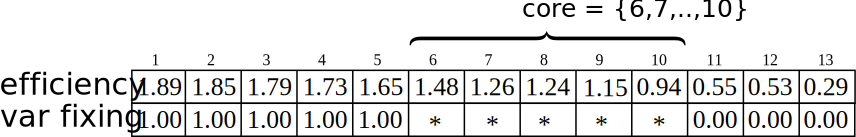
\includegraphics[scale=0.38]{imgs/efficiency} \\
  {\small Example of core for a hypothetical MKP instance.}
\end{center}
For the case of a single constraint (KP) the following efficiency measure can
be considered \vspace{-5pt}
\begin{displaymath}
  e_j = \frac{p_j}{w_j}.
\end{displaymath}
Unfortunately on the MKP there are multiple resources (constraint) to be considered as cost.
Each of then may have different relevance on the cost the item.
This drawback can be avoided by introducing {\bf relevance values} $r_i$
for every constraint:
\begin{displaymath}
  e_j(relevance) = \frac{p_j}{\sum_{i=1}^{m} r_i w_{ij}}
\end{displaymath}
According to \cite{puchinger2006core} setting $r_i$ to the values
of an optimal solution to the dual problem of the MKP's
LP-relaxation, achieves the best results and will be the one
considered in this work.
The optimal solution to the dual problem measures the {\bf scarcity} of that resource

Considering the items in the interval $C = \{ a, \ldots, b \}$ as the core,
the {\bf MKP core problem (MKPC)} can be defined as:
\begin{align}
    \text{maximize} & {\mymathstyle \sum_{j \in C} p_j x_j  + \tilde{p}}\\
    \text{subject to} & {\mymathstyle \sum_{j \in C} w_{ij} x_j \leqslant c_i - \tilde{w}_i, \quad i = 1, \ldots, m}\\
  & x_j \in \{0, 1\}, \quad j \in C.
\end{align}
with $\tilde{p} = \sum^{a-1}_{j=1} p_j$  and $\tilde{w}_i = \sum^{a-1}_{j=1} w_{ij}, i = 1, \ldots, m$
respectively quantifying the total profit and the total weights of items fixed as selected.

This work addresses the development of a SCE metaheuristic applied to MKP core problem.
This hybrid SCE will be referred to as {\bf SCEcr}.

